\documentclass[12pt,addpoints]{exam}
\usepackage{enumitem}
\usepackage{amsfonts,amssymb,amsmath, amsthm}
\usepackage{graphicx}
\usepackage{systeme}
\usepackage{pgf,tikz,pgfplots}
\pgfplotsset{compat=1.15}
\usepgfplotslibrary{fillbetween}
\usepackage{mathrsfs}
\usetikzlibrary{arrows}
\usetikzlibrary{calc}
\pagestyle{headandfoot}
\firstpageheadrule
\runningheader{Grade 10 Chapter 2}{}{Page \thepage\ of \numpages}
\runningheadrule
\author{St John Baptist De La Salle Catholic School, Addis Ababa}
\usepackage{geometry}
\geometry{
	a4paper,
	total={170mm,257mm},
	left=15mm,
	right=15mm,
	bottom=20mm,
	top=15mm,
}
\firstpagefooter{}{}{}
\runningfooter{}{}{}
\date{22/23 Academic Year}

\begin{document}
	\title{Grade 10 Chapter 2 Workbook Questions}
	\maketitle
	
	\begin{center}
		\subsection*{Questions}
	\end{center}
	
	
	\begin{questions}
		\question Why must the test charge $q$ in the definition of the electric field be vanishing small?
		\question Define the following terms and explain what they are.
		\begin{enumerate}[label=(\roman*)]
			\item Charge
			\item Source and test charges
			\item Coulomb Force
			\item Electric field strength
			\item Permittivity of vacuum
			\item Electric potential energy, absolute potential, and voltage
			\item Capacitors
		\end{enumerate}
		\question Why does electrostatic shock almost always happen when touching nonmetallic surfaces?
		\question One important aspect of charge is that it is quantized. How many electrons are needed to form a charge of $-9.6nC$?
		\question Suppose a speck of dust in an electrostatic precipitator has 1.8$\times10^{16}$protons in it and has a net charge of –5.00 nC. How many electrons does it have?
		\question A test charge of $9nc$ is placed halfway between a charge of $-5\mu C$ and another of $9\mu C$ separated by 8 cm.
		\begin{enumerate}[label=(\roman*)]
			\item What is the magnitude and direction of the net electric field due to the charges at the position the test charge is located?
			\item What is the magnitude and direction of the net electric force on the test charge?
		\end{enumerate}
		\question Two point charges of $3\mu C$ and $-7 \mu C$ are placed 40 cm apart.
		\begin{enumerate}[label=(\roman*)]
			\item Where can any test charge be placed such that the net force on the charge due to the point charges above is zero?
			\item What about if both charges were the same parity?
		\end{enumerate}
		\question List the properties of electric lines of force and explain the orientation of the lines in relation with electric field strength.
		\question A simple and common technique for accelerating electrons can be done by separating two plates of opposite charges where there is a uniform electric field between two plates. Electrons are released, usually from a hot filament, near the negative plate, and there is a small hole in the positive plate that allows the electrons to continue moving. If for instance, the field between two plates of a certain apparatus is $2\times10^{5}N/C$, answer the following questions.
		\begin{enumerate}[label=(\roman*)]
			\item What is the acceleration of the electrons?
			\item Why would the electron not be pulled back to the positive plate once it moves through the hole?
		\end{enumerate}
		\question What is the relationship between potential difference and potential energy? Also, express this relationship mathematically.
		\question When measuring voltage, we always measure it between two points. Why is that always the case?
		\question What is the relationship between potential energy and electric field strength?
		\question Show that the units V/m and N/C are the same units.
		\question The electric field strength between two parallel conducting plates separated by 6.00 cm is 7$\times10^{3}$V/m.
		\begin{enumerate}[label=(\roman*)]
			\item What is the potential difference between the two plates?
			\item Assuming the plate with the lowest potential is taken to be at zero volts. What is the potential 2.00 cm from that plate (and 4.00 cm from the other)?
		\end{enumerate}
		\question A 2.00 cm diameter plastic sphere, used in a static electricity demonstration, has a uniformly distributed 40.0 nC charge on its surface. What is the potential near its surface?
		\question What are equipotential lines and surfaces? 
		\begin{enumerate}[label=(\roman*)]
			\item What is distinct about them?
			\item Is work done when moving along equipotential lines? Why? 
			\item Why are equipotential lines perpendicular to electric field lines?
			\item Can different equipotential lines cross? Explain.
		\end{enumerate}  
		\question Based on the Coulomb force, try to explain why capacitance should be proportional to the plate area of a
		capacitor. Similarly, explain why capacitance should be inversely proportional to the separation between plates. 
		\question What is a dielectric? What is the advantage of adding in a dielectric when dealing with capacitors?
		\question If you wish to store a large amount of energy in a capacitor bank, would you connect capacitors in series or parallel?
		\question What application of a physics concept applies on capacitors? Explain how they work
		\question What is time constant? What type of function is the charge as a function of time when a capacitor is charging or discharging?
		\question What capacitance is needed to store $60\mu C$ of charge at a voltage of 120 V?
		\question If the area of the plates of a parallel plate capacitor are doubled while the distance between them is decreased by a factor of 3, by how much does the capacitance change?
		\question What changes can we bring to a capacitor so that it would be able to store more energy?
		\question A parallel plate capacitor has plates of area that are $1.2cm^2$ separated by 0.0200 mm.
		\begin{enumerate}[label=(\roman*)]
			\item What is the capacitance of the capacitor?
			\item How much energy would it be able to store if we apply a voltage of 4V to its plates.
			\item What would its new capacitance be if we added a dielectric of permittivity $\varepsilon=4.40\times10^{-11}F/m$
		\end{enumerate}
		\question Based on the figure shown below, answer the questions that follow.
		\begin{center}
			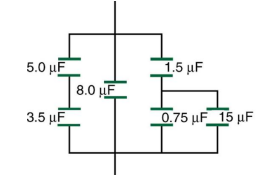
\includegraphics[scale=0.8]{cap}
		\end{center}
		\begin{enumerate}[label=(\roman*)]
			\item Find the effective capacitance of the network.
			\item If we applied a voltage of 6V between the top and bottom ends of the system, calculate the charge and energy stored in each capacitor.
		\end{enumerate}
	\end{questions}		
\end{document}